\documentclass[11pt,a4paper,titlepage]{article}
\usepackage[left=2cm,text={17cm,24cm},top=3cm]{geometry}
\usepackage[T1]{fontenc}
\usepackage[czech]{babel}
\usepackage[utf8]{inputenc}

\usepackage{graphicx}

\usepackage{hyperref} % url

\bibliographystyle{czplain}

%uvozovky
\newcommand{\ceskeuvozovky}[1]{\quotedblbase#1\textquotedblleft}
\begin{document}

\begin{titlepage}
\begin{center}
    {\LARGE\textsc{Vysoké učení technické v~Brně}}\\
    \smallskip
    {\Large\textsc{Fakulta informačních technologií}}\\
    \bigskip
    \vspace{\stretch{0.382}}
    \LARGE{Modelování a simulace - projekt}\\
    \smallskip
    \Huge{Produkce řepky v ČR}\\
    \vspace{\stretch{0.618}}
\end{center}
    {\Large Petr Kapoun - xkapou04 \\ Erik Kelemen - xkelem01 \hfill \today }
\end{titlepage}

\tableofcontents
\newpage


\section{Úvod}
I like IMS. I want A. I not nice when not A. I kill garant when not A. Give A.


\section{Postřiky}
Za dobu blah blah. Zvolili jsme kompletní řešení postřiků od fitmy BASF\footnote{BASF je německá agrochemická firma, která patří k 
největším na světě.\\https://www.agro.basf.cz/agroportal/cz/cs/startpage.html.}.
Pro určení přibližné ceny jednotlivých postřikových přípravků použijeme ceny existujícího eshopu obchod.agrokop.cz\footnote{AGROKOP CZ, a.s. Třebíč}.
\begin{figure}[ht!]
\centering
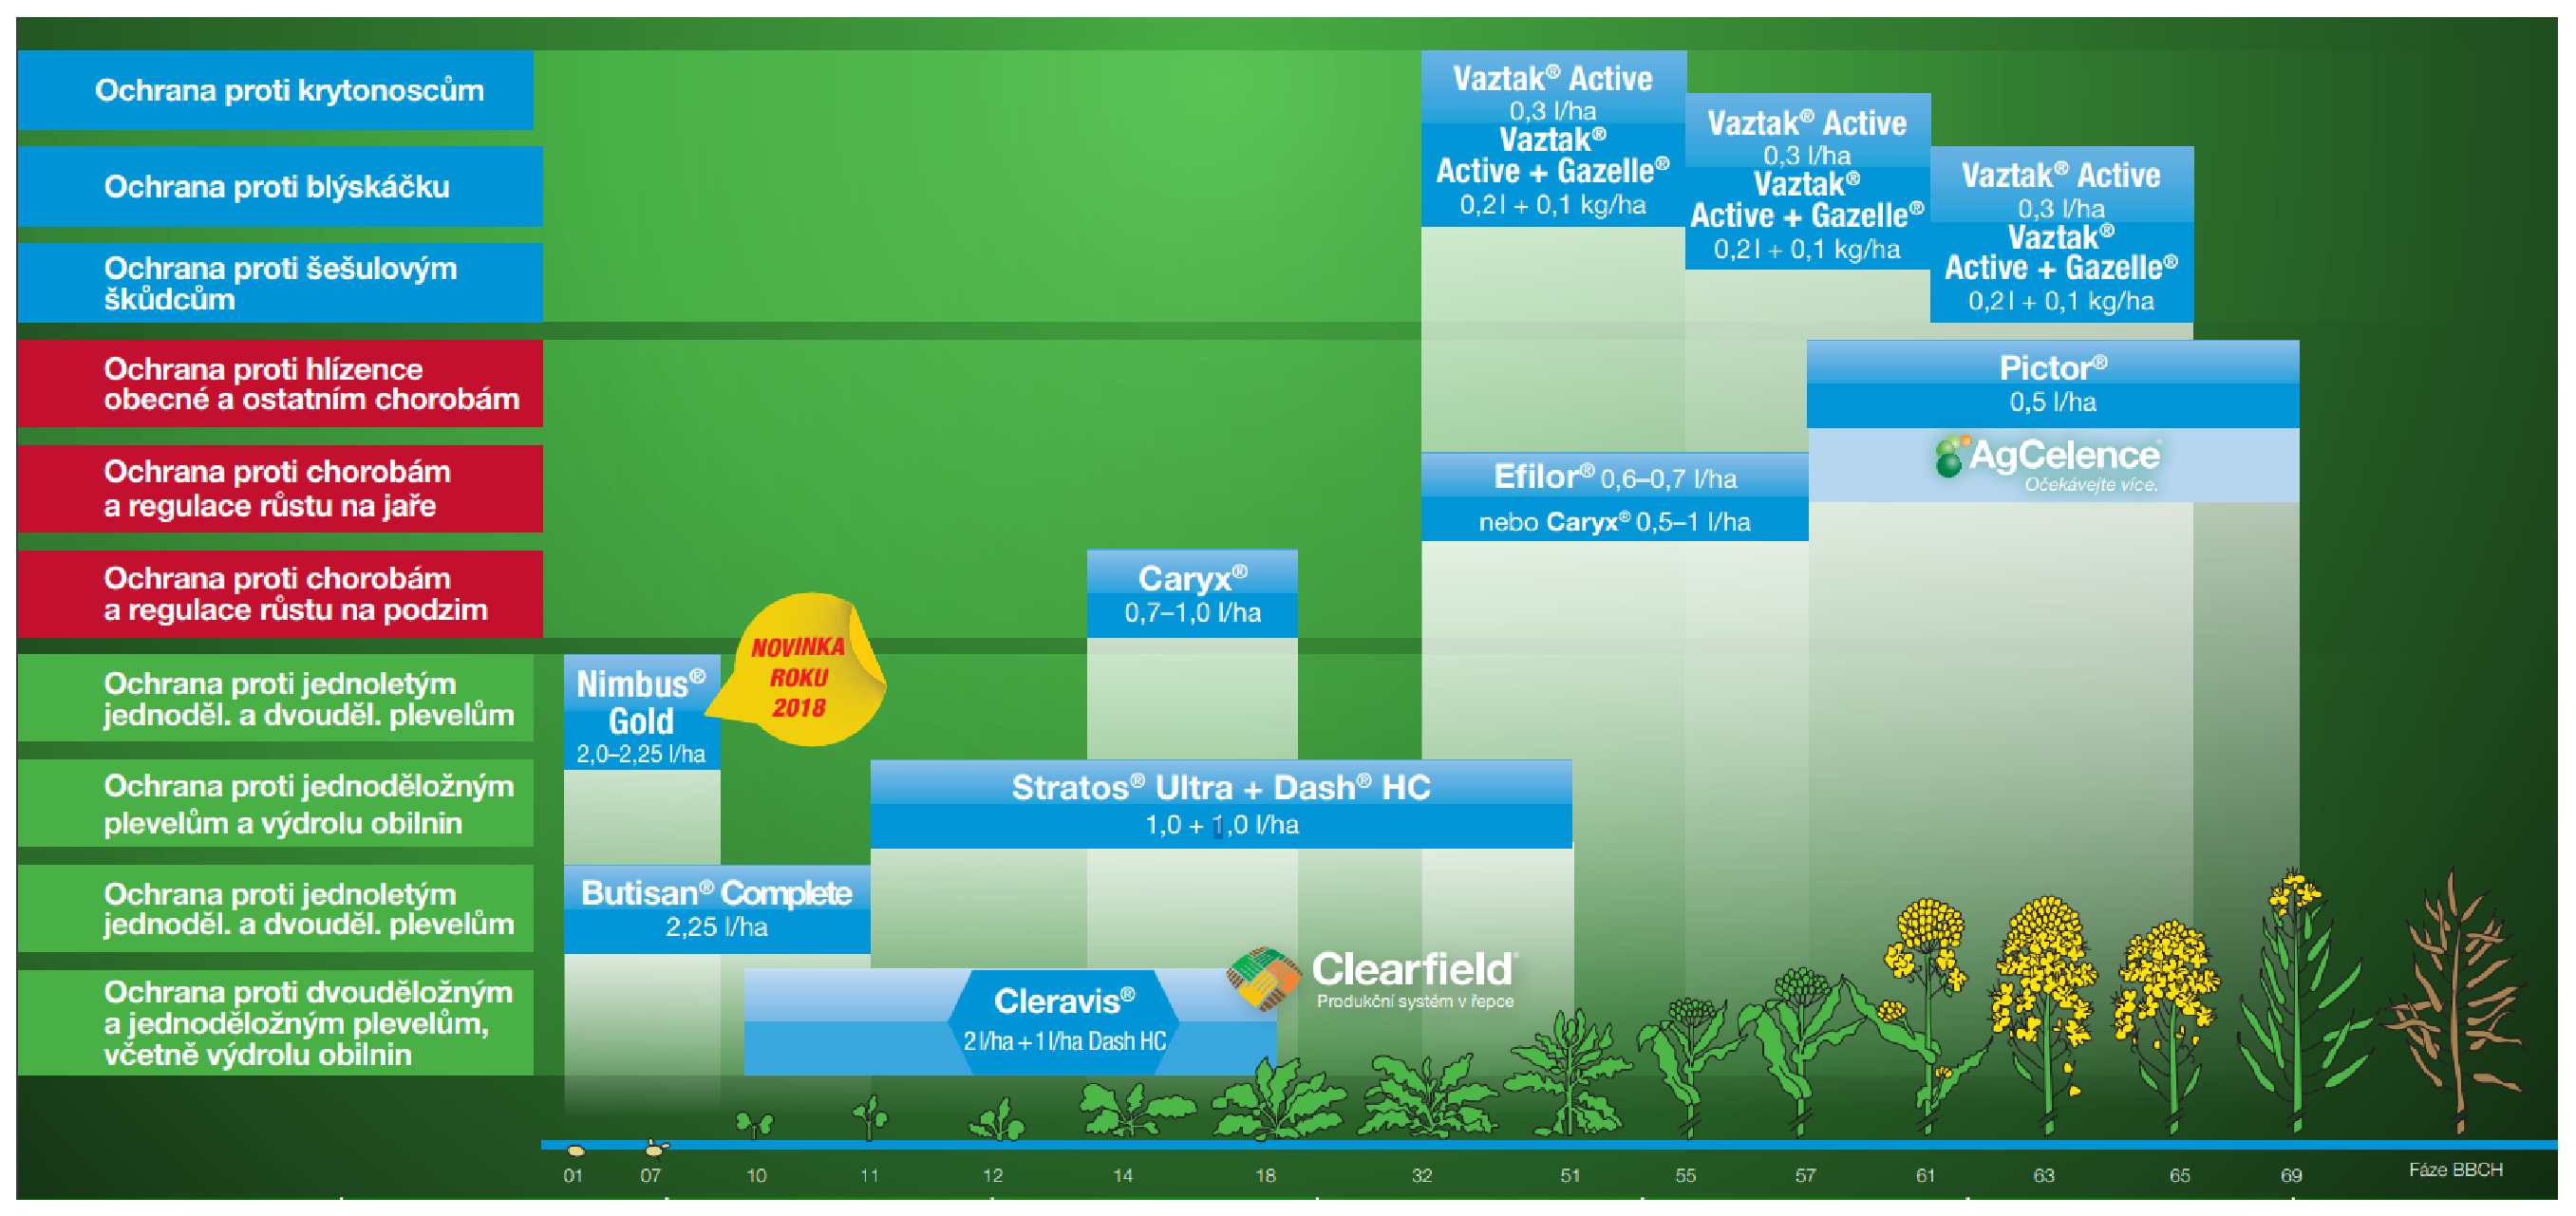
\includegraphics[width=170mm]{img/basf_postriky.eps}
\caption{Ochrana řepky proti škodlivým činitelům firmy BASF \label{overflow}}
\end{figure}
Používané přípravky se dělí do několika skupin, to je důležité hlavně kvůli informaci o mísitelnosti jednotlivých přípravků.
\begin{itemize}
  \item Listová hnojiva.
  \item Fungicidy.
  \item Insekticidy.
  \item Herbicidy.
  \item Graminicidy.
\end{itemize}

\subsection{Ochrana proti krytonoscům, blýskáčku a šešulovým škůdcům}
Použitý přípravek se nazývá Vaztak Active\footnote{Vaztak je přípravek německého výrobce BASF: \\\url{\detokenize{
https://www.agro.basf.cz/agroportal/cz/cs/crop_protection/vyhled_v_n__p__pravk__podle_parametr_/product_details_24923.html
}}.}.
\begin{itemize}
  \item Spotřeba 0,3l/ha. * 3 za každé období postřiku.
  \item Doporučené množství vody 200–600 l/ha (polní plodiny, zelenina), 200–1000 l/ha (prostorové plodiny) 
  \item Kategorie Insekticidy.
  \item Mísit lze se vším.
  \item Cena 815 bez DPH za litr.
\end{itemize}

\subsection{Ochrana proti hlízence obecné a ostatním chorobám}
Použitý přípravek se nazývá Pictor\footnote{Pictor je přípravek německého výrobce BASF: \\\url{\detokenize{
https://www.agro.basf.cz/agroportal/cz/cs/crop_protection/vyhled_v_n__p__pravk__podle_parametr_/product_details_1396.html
}}.}.
\begin{itemize}
  \item Spotřeba 0,5l/ha.
  \item Doporučené množství vody 200-400l.
  \item Kategorie Fungicidy.
  \item Mísit lze se vším.
  \item Cena 3280 bez DPH za litr.
\end{itemize}

\subsection{Ochrana proti chorobám a regulace růstu na jaře}
Použitý přípravek se nazývá Efilor\footnote{Efilor je přípravek německého výrobce BASF: \\\url{\detokenize{
https://www.agro.basf.cz/agroportal/cz/cs/crop_protection/vyhled_v_n__p__pravk__podle_parametr_/product_details_72192.html
}}.}.
\begin{itemize}
  \item Spotřeba 0,6l/ha.
  \item Doporučené množství vody 150-400l.
  \item Kategorie Fungicidy.
  \item Mísit nelze pouze pýrohubné dávky u Graminicidů.
  \item Cena 1399 bez DPH za litr.
\end{itemize}
Efilor zajišťuje vynikající ochranu proti houbovým chorobám a kompaktní porosty s ideální architekturou, které díky tomu rovnoměrně kvetou a dozrávají.

\subsection{Ochrana proti chorobám a regulace růstu na podzim}
Použitý přípravek se nazývá Caryx\footnote{Caryx je přípravek německého výrobce BASF: \\\url{\detokenize{
https://www.agro.basf.cz/agroportal/cz/cs/crop_protection/vyhled_v_n__p__pravk__podle_parametr_/product_details_1446.html
}}.}.
\begin{itemize}
  \item Spotřeba 0,75-1l/ha.
  \item Doporučené množství vody 150-400l.
  \item Kategorie Fungicidy.
  \item Mísit nelze pouze pýrohubné dávky u Graminicidů.
  \item Cena 1009 bez DPH za litr.
\end{itemize}

\subsection{Ochrana proti jednoletým jednoděl. a dvouděl. plevelům}
První možný přípravek se nazývá Butisan Complete\footnote{Butisan Complete je přípravek německého výrobce BASF: \\\url{\detokenize{
https://www.agro.basf.cz/agroportal/cz/cs/crop_protection/vyhled_v_n__p__pravk__podle_parametr_/product_details_85632.html
}}.}.
\begin{itemize}
  \item Spotřeba 2-2,25l/ha.
  \item Doporučené množství vody 100-400l.
  \item Kategorie Herbicidy.
  \item Mísit lze se vším.
  \item Cena 1016 bez DPH za litr.
\end{itemize}

Druhý možný přípravek se nazývá Nimbus Gold\footnote{Nimbus Gold je přípravek německého výrobce BASF: \\\url{\detokenize{
https://www.agro.basf.cz/agroportal/cz/cs/crop_protection/vyhled_v_n__p__pravk__podle_parametr_/product_details_99459.html
}}.}.
\begin{itemize}
  \item Spotřeba 2-2,25l/ha.
  \item Doporučené množství vody 100-400l.
  \item Kategorie Herbicidy.
  \item Mísit lze se vším.
  \item Cena 919 bez DPH za litr.
\end{itemize}

\subsection{Ochrana proti jednoděložným plevelům a výdrolu obilnin}
Použitý přípravek se nazývá Stratos Ultra\footnote{Stratos Ultra je přípravek německého výrobce BASF: \\\url{\detokenize{
https://www.agro.basf.cz/agroportal/cz/cs/crop_protection/vyhled_v_n__p__pravk__podle_parametr_/product_details_1429.html
}}.}.
\begin{itemize}
  \item Spotřeba 1l/ha.
  \item Doporučené množství vody 200-300l.
  \item Kategorie Herbicidy.
  \item Mísit nelze s listovým hnojivem Solubor.
\end{itemize}
Pomocný přípravek se nazývá Dash HC\footnote{Dash HC je přípravek německého výrobce BASF: \\\url{\detokenize{
https://www.agro.basf.cz/agroportal/cz/cs/crop_protection/vyhled_v_n__p__pravk__podle_parametr_/product_details_1441.html
}}.}.
\begin{itemize}
  \item Spotřeba 1l/ha.
  \item Doporučené množství vody 300.
\end{itemize}
Cena za 10l přípravku Stratos Ultra a 10l přípravku Dash HC je 6990 bez DPH.

\subsection{Ochrana proti dvouděložným a jednoděložnám plevelům, včetně výdrolu obilnin}
Použitý přípravek se nazývá Cleravis\footnote{Cleravis je přípravek německého výrobce BASF: \\\url{\detokenize{
https://www.agro.basf.cz/agroportal/cz/cs/crop_protection/vyhled_v_n__p__pravk__podle_parametr_/product_details_55941.html
}}.}.
\begin{itemize}
  \item Spotřeba 2l/ha.
  \item Doporučené množství vody 300-400l.
  \item Kategorie Herbicidy.
  \item Mísit nelze s Graminicidy.
\end{itemize}
Pomocný přípravek se nazývá Dash HC.
\begin{itemize}
  \item Spotřeba 1l/ha.
  \item Doporučené množství vody 300.
\end{itemize}
Cena za 10l přípravku Cleravis a 5l přípravku Dash HC je 11699 bez DPH.


\section{Voda}
Vodu ukradneme z potoka.


\section{Hnojiva}
Těžký business, ceny nejsou veřejné.


\section{Zemědělské stroje}
Kombajn, traktor, levný nezaměstnaný podivín.


\section{Hledání informací}
U~informací, které používáme ve~svých pracích, je~potřeba kontrolovat jejich správnost. V~mnoha případech je~samozřejmě situace méně jasná a~rozdílné názoty ilustrují, že~zde může být konfliktní pohled na~pravdu a~falešnost.\cite{Ar_Information}


\section{Textové sdílení informací}
V~moderní kultuře lidé méně mluví a~více píší . Nemám na~mysli rukopis, ale~textování a~psaní na~stroji.
\cite{Ar_Luv2TxT}
\textit{„Tištěná média mají dlouhou tradici, odvíjející se od~letáků, jednolistých prohlášení a~rozsáhle šířených krátkých polemik.“}\cite{Douda_informace} I~my dnes potřebujeme předat některé informace formou textu, příkladem může být elektronická pošta. U~některých rozsáhlejších textů, jako jsou manuály, bakalářské a~diplomové práce, je~nutné dodržovat strukturu textu a~další konvence. V~mnoha věcech nám pomůže znalost typografie. K~prezentaci vlastních myšlenek nám~může pomoci například sázecí prostředí. \LaTeX .


\section{Co~je~\LaTeX?}
Totální HOVNO, ale lze říci, že~prakticky neexistuje osobní počítač, na~němž by~nebyl k~dispozici textový editor nebo některý z~produktů kategorie DTP - Desk Top Publishing (publikování "na~stole"). \cite{RybickaLatex}
Latex je~generický sázecí systém, který používá tex jako svůj formátovací stroj.\cite{Latex_companion} Jedná se~o~velice elegantní sérii příkazů, které posílají naše myšlenky sázecímu systému, který poté vytvoří dokument pro~naše potěšení.\cite{programujte}
Díky své flexibilitě, lehkosti použití a~profesionální typografické kvalitě je~momentálně \LaTeX používán skoro ve~všech humanitních oblastech a~ve~vědě.\cite{Latex_companion}


\newpage
\bibliography{literatura}

\end{document}
